\chapter{Sztuczna inteligencja - rozdział teoretyczny}
\label{cha:ogolnyrozdzialteoretyczny}

Jednym z najistotniejszych zagadnień z dziedziny sztucznej inteligencji jest uczenie maszynowe. 


\section{Uczenie maszynowe}

Uczenie maszynowe jest metodą analizy danych, która automatyzuje budowę modelu analitycznego na podstawie nauki z 
danych. W wielu zastosowaniach ich użycie jest znacznie bardziej efektywne od manualnego programowania, w wyniku czego 
uczenie maszynowe znalazło szerokie zastosowanie w informatyce i innych dziedzinach.
W ostatniej dekadzie można zauważyć zwiększone użycie metod uczenia maszynowego\cite{domingos2012few}.

\section{Podejścia do uczenia maszynowego}
\label{sec:podejsciadouczeniamaszynowego}

\begin{itemize}
 \item uczenie nadzorowane,
 \item uczenie nienadzorowane,
 \item uczenie ze wzmocnieniem,
\end{itemize}

\subsection{Uczenie nadzorowane}
\label{subsec:uczenienadzorowane}

Uczenie nadzorowane polega na wnioskowaniu funkcji z określonych danych treningowych.
Wykorzystując dostarczone przykłady algorytmy potrafią estymować wartości danych, które mogą nie występować w 
podanym zbiorze wejściowym. Dzięki generalizowaniu z przykładów, metody uczenia nadzorowanego są w stanie 
wyznaczać przewidywane wartości na podstawie danych trenujących.

Ważną cechą danych trenujących w uczeniu nadzorowanym jest konieczność ich oznaczenia. Algorytm, aby móc 
szacować pożądane wartości funkcji, musi posiadać wiedzę o ich cechach.

Przykładem zastosowania algorytmów uczenia nadzorowanego jest system rozpoznawania niechcianych wiadomości w klientach 
pocztowych. Danymi wejściowymi są w tym przypadku kategoryzowane na pożądane lub niepożądane wiadomości e-mail.
System generalizując podane mu przykłady jest w stanie zidentyfikować kolejne wiadomości i wykonać odpowiednią akcję, 
zależnie od preferencji użytkownika (może to być na przykład usunięcie lub przeniesienie do zdefiniowanego folderu).

Wiele różnych algorytmów uczenia nadzorowanego zostało wykorzystanych by rozwiązać problem klasyfikacji wiadomości 
e-mail. Użyto między innymi algorytmów k-nearest neighbor\cite{firte2010spam}, Naive 
Bayes\cite{marsono2008binary}\cite{lakshmi2010spam} czy Random Forest\cite{koprinska2007learning}, jednak wiąże 
się to z istotnymi wadami\cite{li2014towards}:

\begin{itemize}
 \item \textbf{Wymagane oznaczenie danych testowych}. Metody uczenia nadzorowanego wymagają, aby dane trenujące były 
oznaczone. W przypadku klasyfikacji wiadomości e-mail, koniecznie jest ich oznaczenie w zależności od tego czy są 
szkodliwe czy nie. Problem stwarza tutaj wielkość danych. Ilość wiadomości, która jest wymieniana w sieci jest 
bardzo duża. W związku z czym, żeby klasyfikacja miała sens, wymagane też jest oznaczenie sporej ilości przykładów, co 
nie zawsze jest możliwe i opłacalne do zrealizowania. 
\item \textbf{Mała liczba danych testowych}. W związku z niewielką (w stosunku do wszystkich możliwych) ilością danych 
trenujących, algorytm jest mało odporny na modyfikowane dane. Osoby rozsyłające niechciane wiadomości bardzo często 
będą zmieniać ich treść i strukturę, na taką, która nigdy nie pojawiła się wśród danych trenujących. Może mięc to 
negatywny wpływ na wynik działania algorytmu.
\end{itemize}


 

\subsection{Uczenie nienadzorowane}
\label{subsec:uczenienienadzorowane}

Podobnie jak w uczeniu nadzorowanym, algorytmy uczenia nienadzorowanego wyznaczają funkcje na podstawie danych 
wejściowych, jednak są w stanie odkryć niewidoczne zależności między nimi. Konsekwencją wynikającą z charakterystyki 
danych trenujących jest niemożność określenia błędu lub poprawności rozwiązania. Celem działania algorytmu może być na 
przykład kategoryzowanie informacji (klasteryzacja).

Metody uczenia nienadzorowanego są w stanie wykryć wzorzec w danych wejściowych


\subsection{Uczenie ze wzmocnieniem}
\label{subsec:uczeniezewzmocnieniem}




\section{Podsumowanie}


\section{Przykład zastosowania algorytmów uczenia maszynowego}
\label{sec:przykladzastosowaniaalgorytmowuczeniamaszynowego}

Używając jako wejścia informacji dotyczących kwiatów irysów, w przedstawionej poniżej postaci, algorytmy uczenia 
nienadzorowanego są w stanie przewidzieć gatunek kwiatu (\textit{setosa}, \textit{versicolor},  \textit{virginica}) na 
podstawie długości i szerokości płatka  (\textit{sepal}) i listka kielichu (\textit{petal}).

\begin{code}[caption=Przykład danych dotyczących kwiatów irysów, label=amb, captionpos=b, belowcaptionskip=4pt]
    Sepal.Length Sepal.Width Petal.Length Petal.Width    Species
1            5.1         3.5          1.4         0.2     setosa
2            4.9         3.0          1.4         0.2     setosa
3            4.7         3.2          1.3         0.2     setosa
4            4.6         3.1          1.5         0.2     setosa
53           6.9         3.1          4.9         1.5 versicolor
54           5.5         2.3          4.0         1.3 versicolor
55           6.5         2.8          4.6         1.5 versicolor
56           5.7         2.8          4.5         1.3 versicolor
101          6.3         3.3          6.0         2.5  virginica
102          5.8         2.7          5.1         1.9  virginica
103          7.1         3.0          5.9         2.1  virginica
104          6.3         2.9          5.6         1.8  virginica
\end{code}
\\\\\\
Na ryc. ~\ref{fig:plotsepalwidthsepallength}, przedstawione zostało rozmieszczenie gatunków kwiatów w zależności od 
długości i szerokości płatka kwiatu. Wyraźnie widać podział na dwa podstawowe klastry
\begin{itemize*} 
\renewcommand{\labelitemi}{$\bullet$}
 \item gatunek setosa,
 \item gatunek versicolor i virginica.
\end{itemize*}

\begin{figure}[b]
    \centering
    \textbf{Rozmieszczenie kwiatów irysów}\par\medskip
    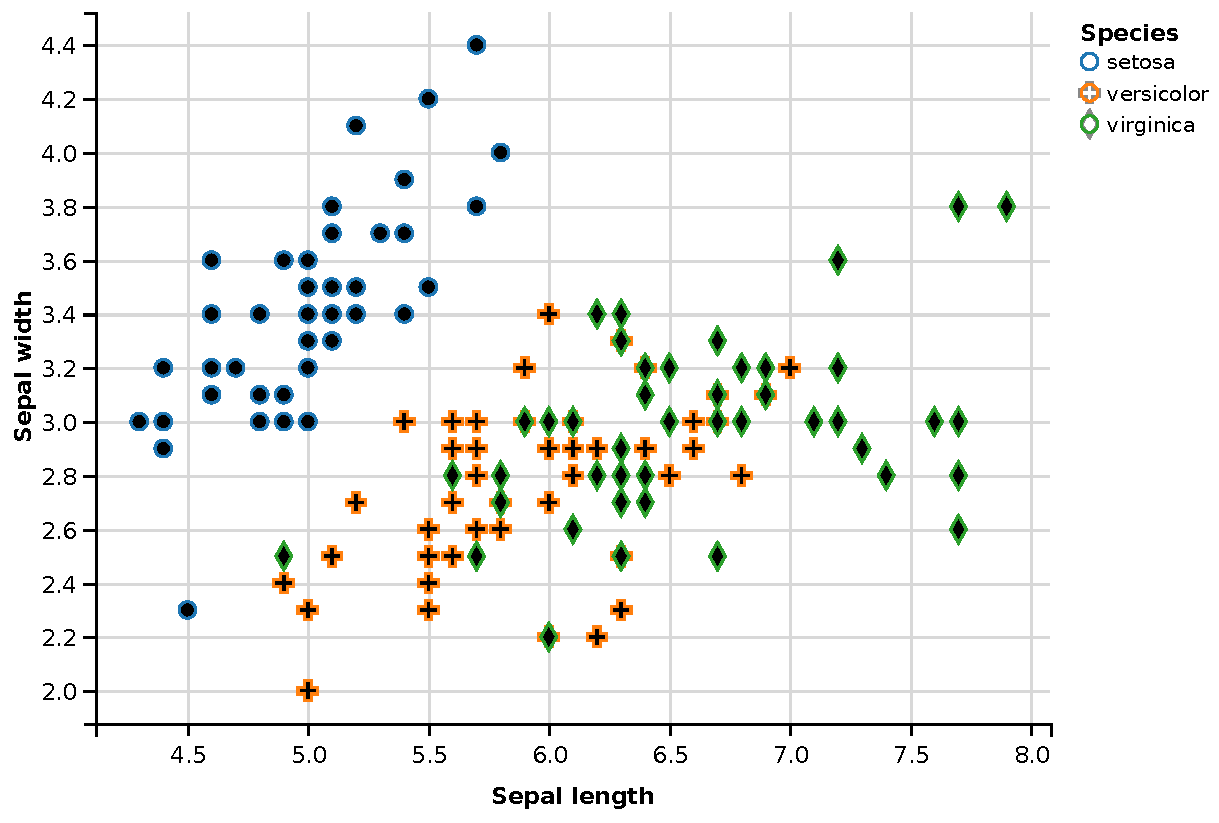
\includegraphics[scale=0.7]{plotsepalwidthsepallength}
    \caption{Populacja kwiatów irysów w zależności od szerokości i długości płatka kwiatu. Źródło: Opracowanie własne}
    \label{fig:plotsepalwidthsepallength}
\end{figure}















